\section{Páronkénti konnektivitás}\label{sec:PAIRWISE_CONNECTIVITY}
Egycélú CNDP esetén a kihívás abban áll, hogy találjunk egy olyan konnektivitási metrikát,
amely alkalmazási területtől függően megfelelően leírja egy gráf összefüggőségét.
$S$-el fogjuk jelölni a törlendő csomópontok halmazát,
míg az$f(S)$ jóság függvény fogja jellemezni a $G[V \setminus S]$ feszített részgráf összefüggőségét.
Ha $H$-val jelöljük a $G[V \setminus S]$ feszített részgráf összefüggő komponenseinek a halmazát,
akkor a jóság függvény a következő képlettel írható le:
\begin{equation}\label{eqn:PAIRWISE_CONNECTIVITY}
  f(S) = \sum_{h \in H} \frac{\abs{h} \cdot (\abs{h} - 1)}{2},
\end{equation}
amelyet az irodalom \cite{ventresca2012global, aringhieri2016general} úgy tart számon,
hogy \textbf{páronkénti konnektivitás}.
Tehát a feladat \aref{eqn:PAIRWISE_CONNECTIVITY} függvénynek a minimalizálása:
\begin{equation}\label{eqn:MIN_PAIRWISE_CONNECTIVITY}
  \min_{S \subseteq V} f(S).
\end{equation}

\Aref{eqn:PAIRWISE_CONNECTIVITY} fitnesz függvény implementációját \aref{lst:PAIRWISE-CONNECTIVITY}. kódrészlet szemlélteti Python-ban.
\lstinputlisting[
  language={Python},
  caption={Páronkénti konnektivitás},
  label={lst:PAIRWISE-CONNECTIVITY}
]{./progfiles/single-objective-cndp/pairwise_connectivity.py}


\subsubsection{Egy példa}
\Aref{fig:PAIRWISE_CONNECTIVITY_EXAMPLE}. ábrán látható gráfban,
ha $k = 2$ kritikus csomópontot kell azonosítanunk,
akkor $S = \left\{ 1, 2 \right\}$ eredményezi az optimális megoldást.
A $G\left[ V \setminus S \right]$ feszített részgráf két, egyenként öt csomópontból álló összefüggő komponensre esik szét,
vagyis $\abs{H} = 2$. Így \aref{eqn:PAIRWISE_CONNECTIVITY} jóság függvény a következőképpen számolódik:
\[
  f(S) = \dfrac{5 - (5 - 1)}{2} + \dfrac{5 - (5 - 1)}{2} = 20
\]

\begin{figure}[h]
  \centering
  \begin{tabular}{ll}
    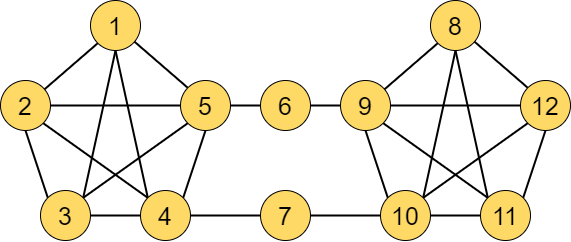
\includegraphics[scale=0.3]{images/pairwise_connectivity_before.png}
     &
    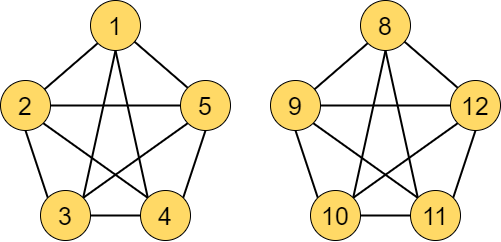
\includegraphics[scale=0.3]{images/pairwise_connectivity_after.png}
  \end{tabular}
  \caption{
    Példa egy kis méretű gráfra (bal oldalt), amely a 6. és 7. csomópontok törlése után
    szétesik két összefüggő komponensre (jobb oldalt).
  }
  \label{fig:PAIRWISE_CONNECTIVITY_EXAMPLE}
\end{figure}
